\documentclass{article}
\usepackage{pdfpages}
\setcounter{section}{-2}

%\usepackage{fancyhdr}
%\pagestyle{fancy}
%\fancyhf{}
%\renewcommand{\headrulewidth}{0pt}
%\fancyhead[R]{\thepage}


\usepackage{fancyhdr}


\begin{document}

\title{SCMA248 Introduction to Data Science}
\author{Pairote Satiracoo}
\maketitle


\tableofcontents 
\newpage

\section{Course Syllabus}
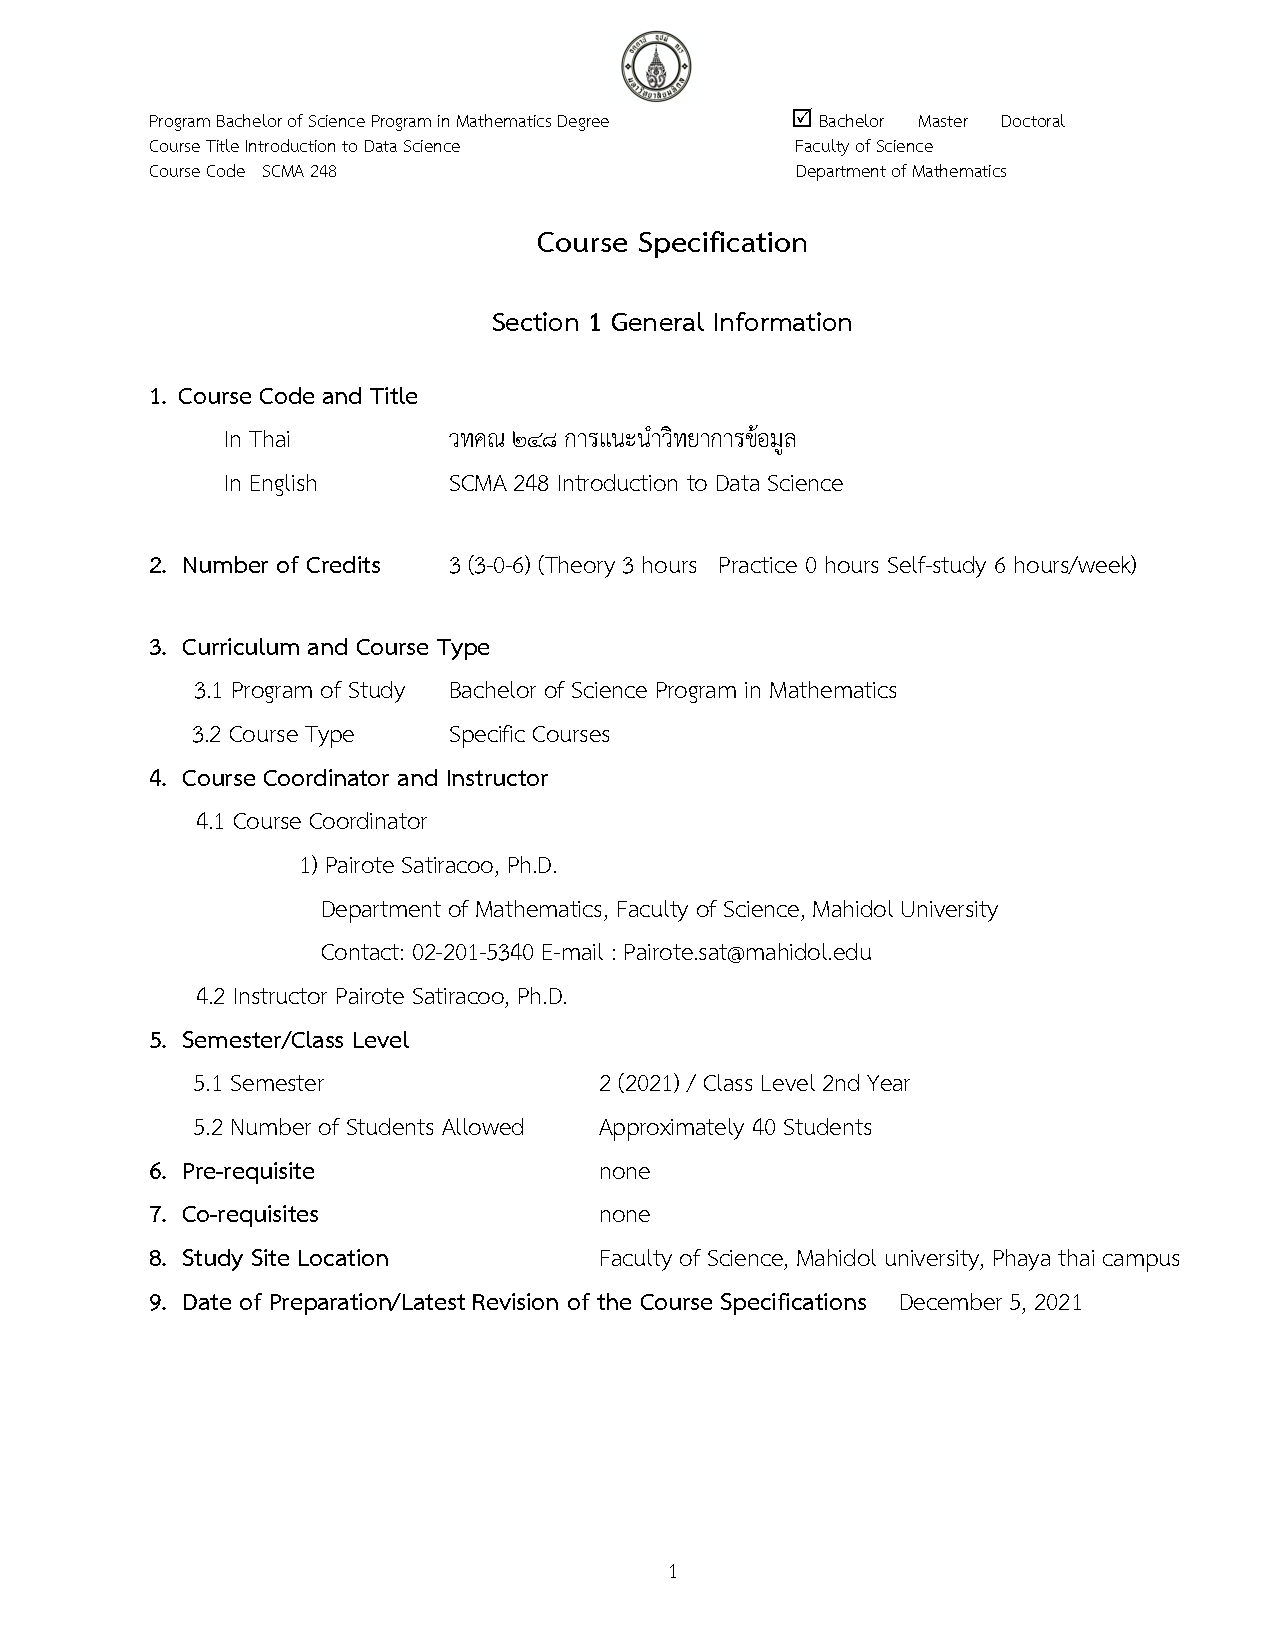
\includepdf[pages={1-},scale=0.8,pagecommand={\thispagestyle{plain}}, angle=0]{SyllabusSCMA248-2021}

\section{Welcome to SCMA248 Introduction to Data Science}
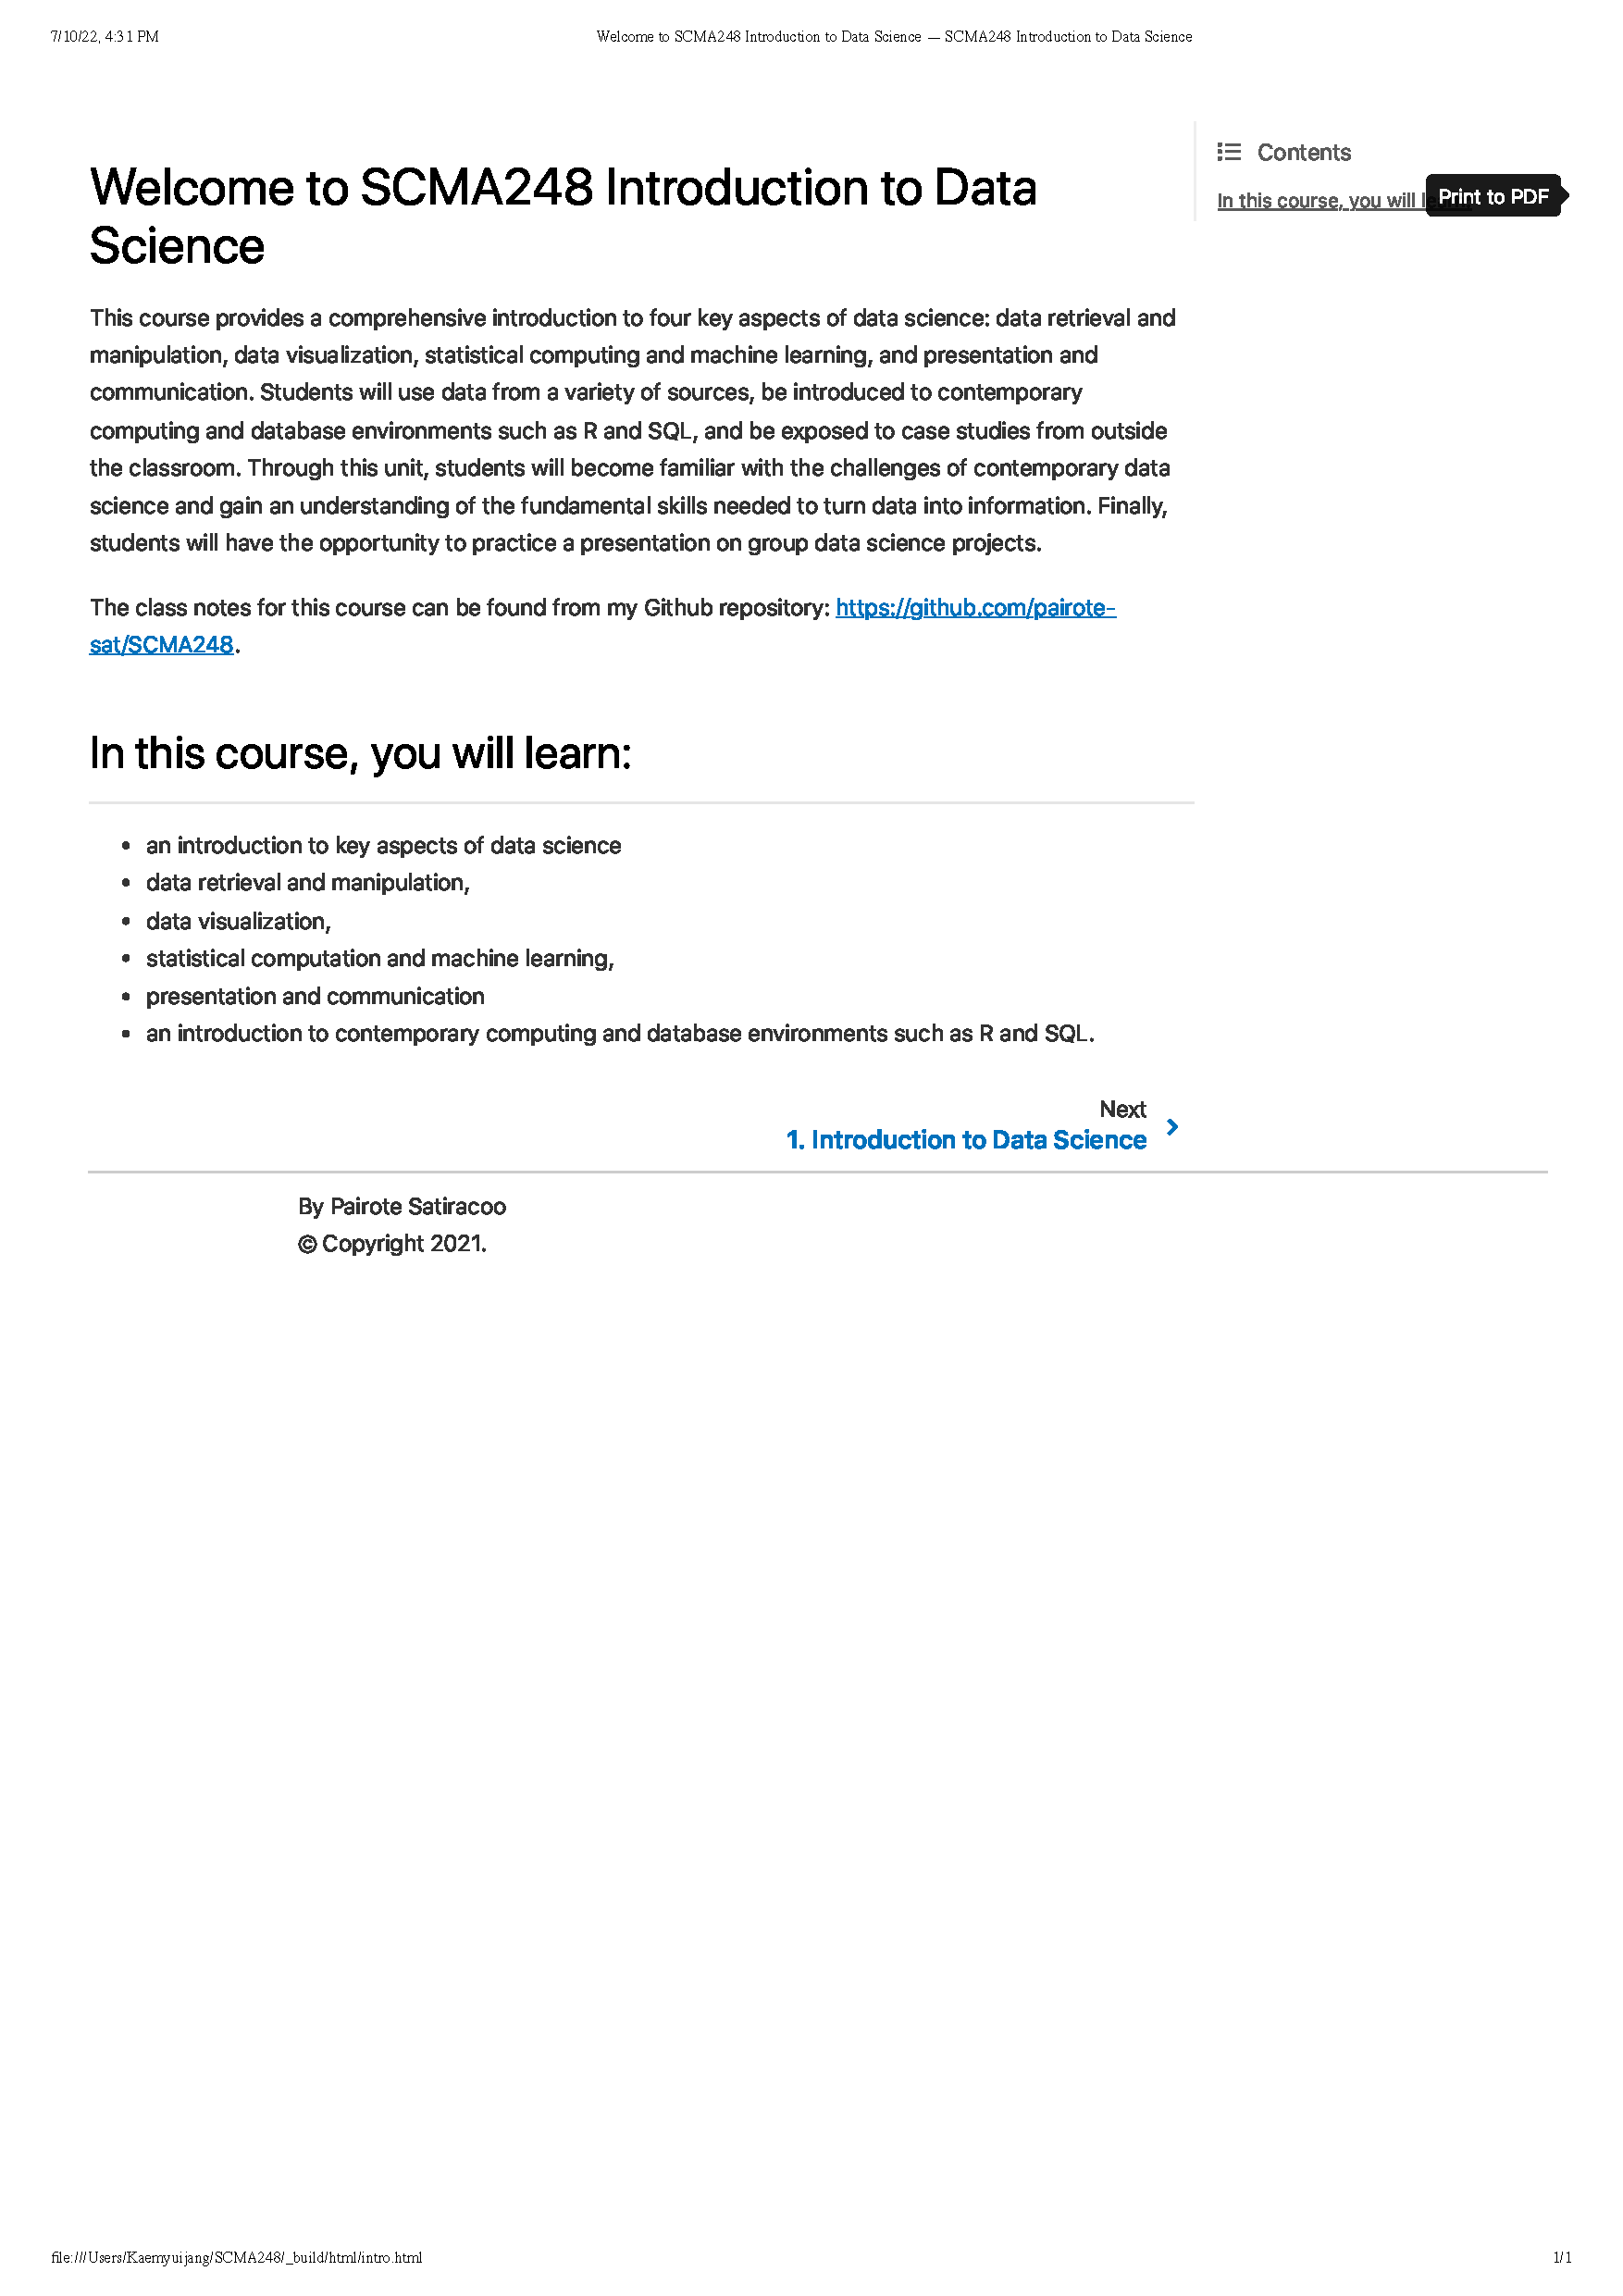
\includepdf[pages={1-},scale=0.8,pagecommand={\thispagestyle{plain}}, angle=0]{0Welcome.pdf}
\section{Introduction to Data Science}
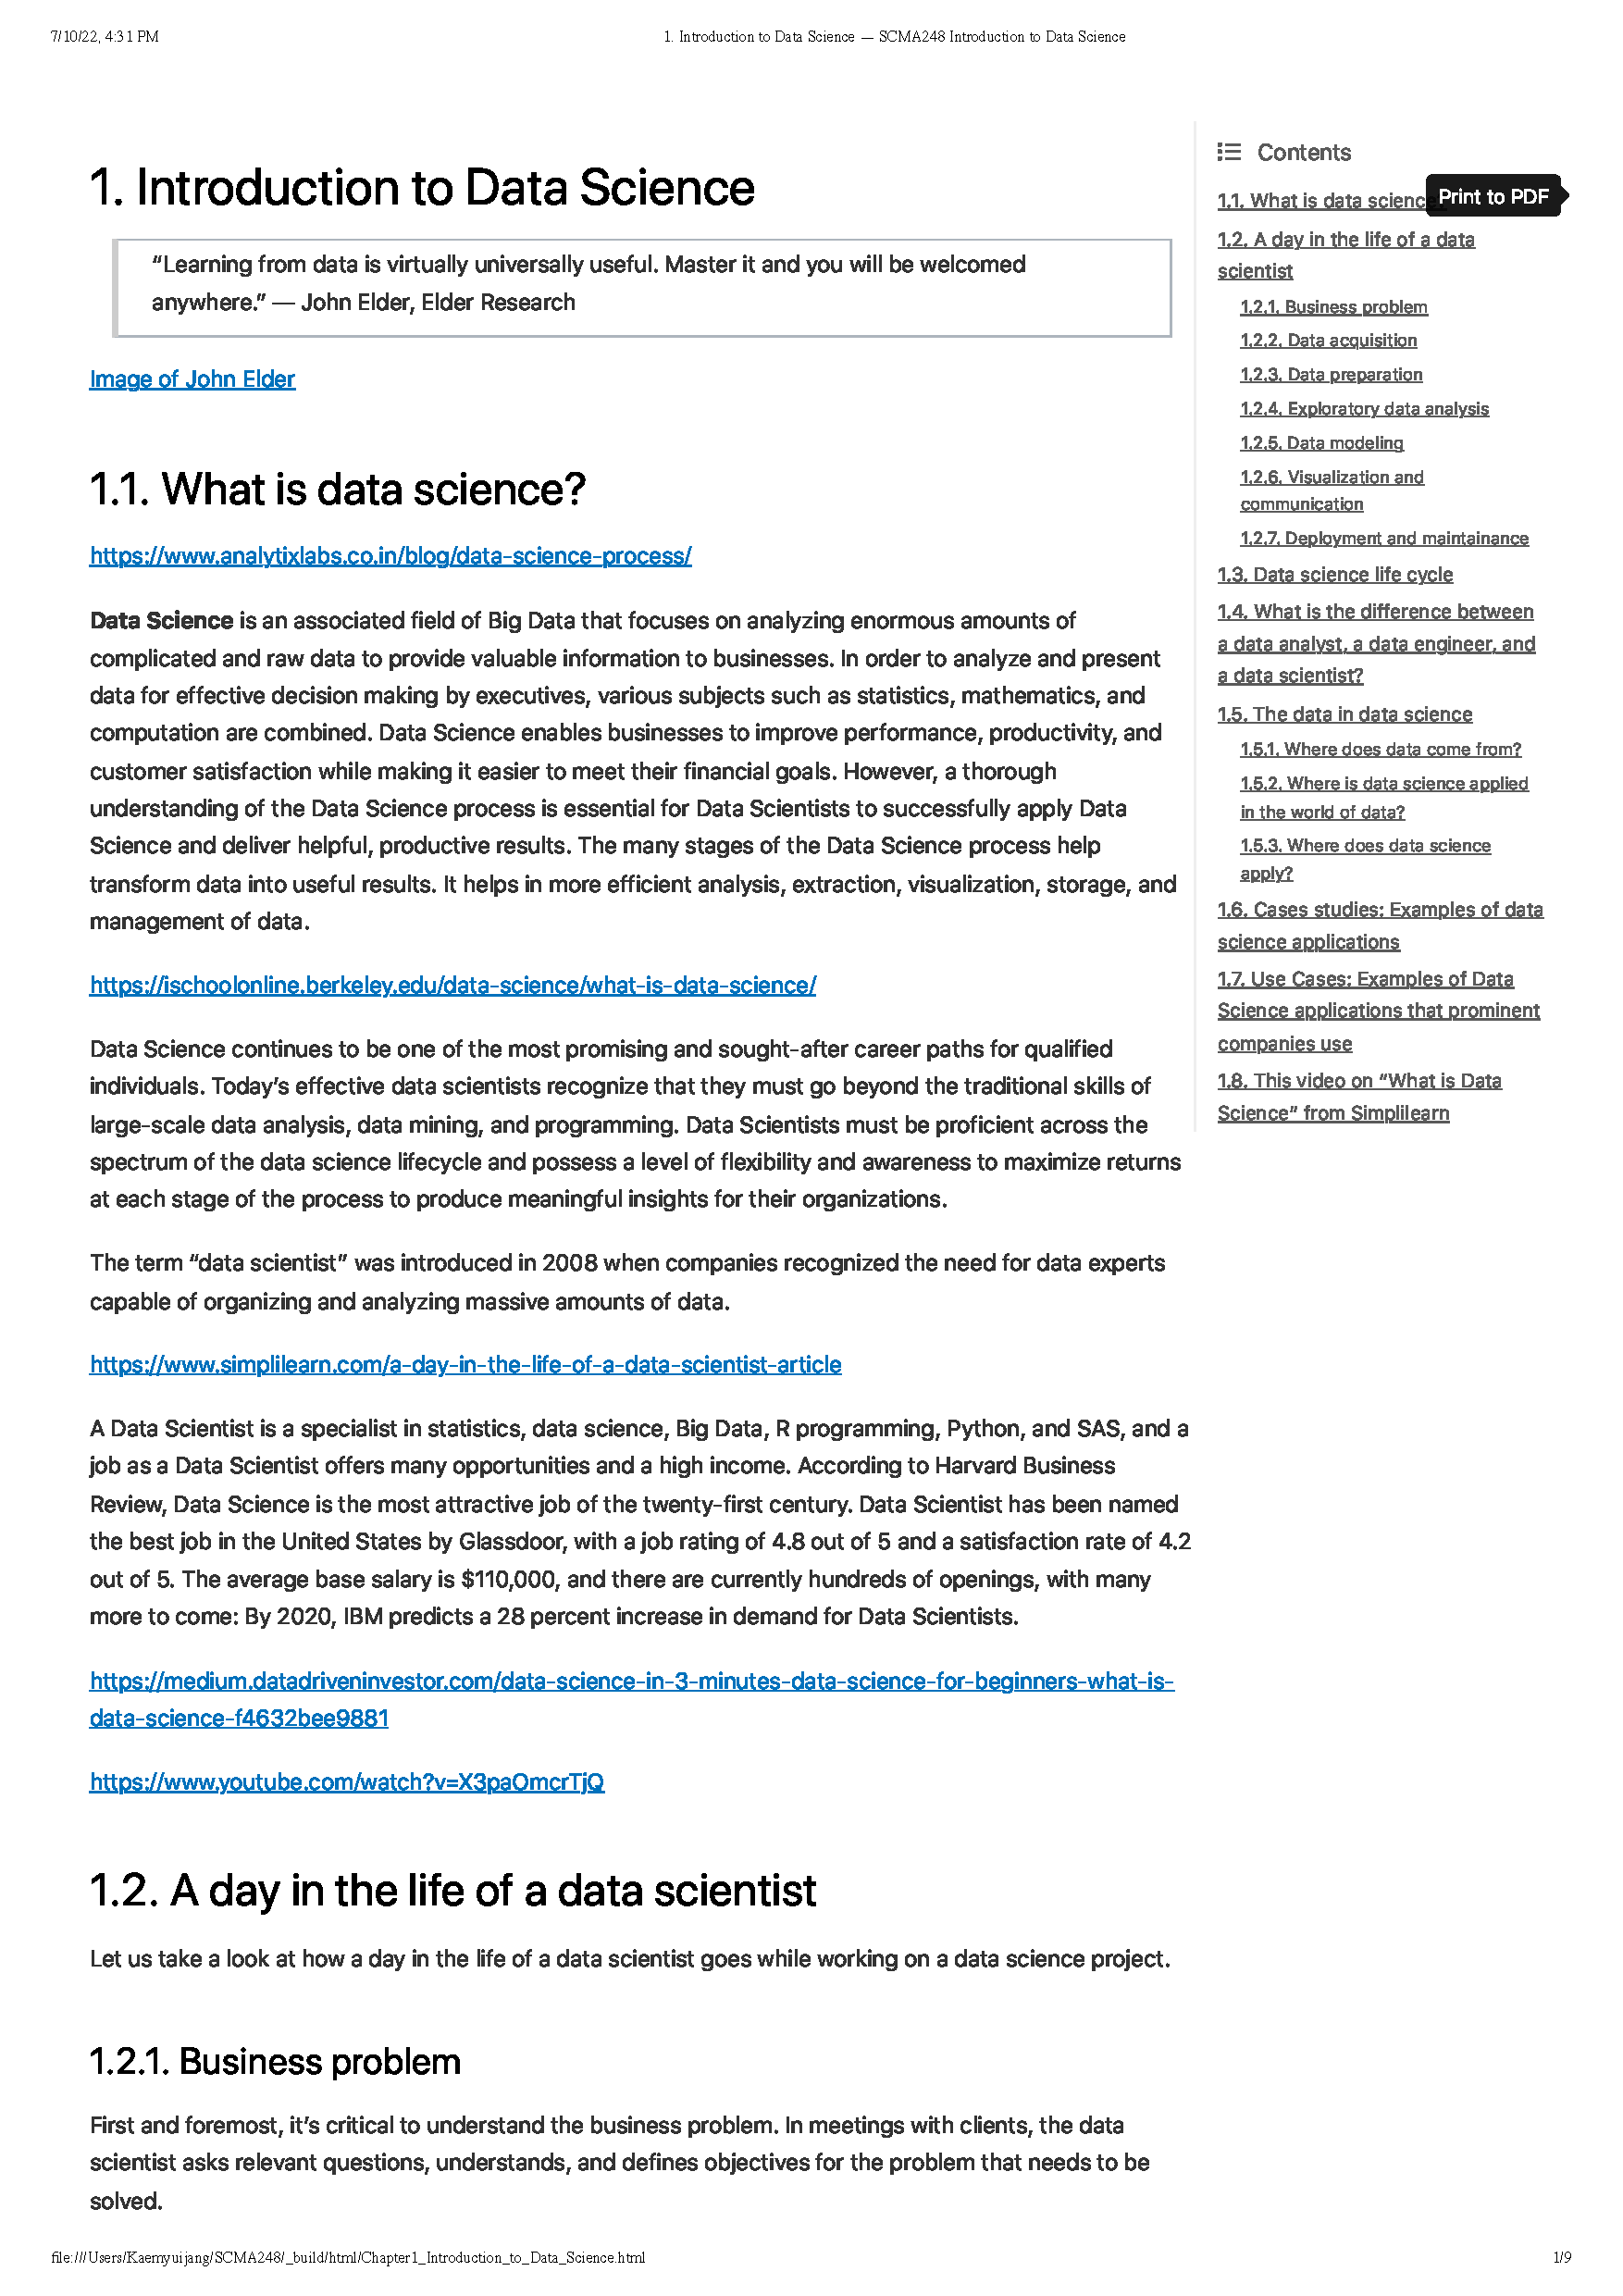
\includepdf[pages={1-},scale=0.8,pagecommand={\thispagestyle{plain}}, angle=0]{1Introduction.pdf}
\section{Python Basics}
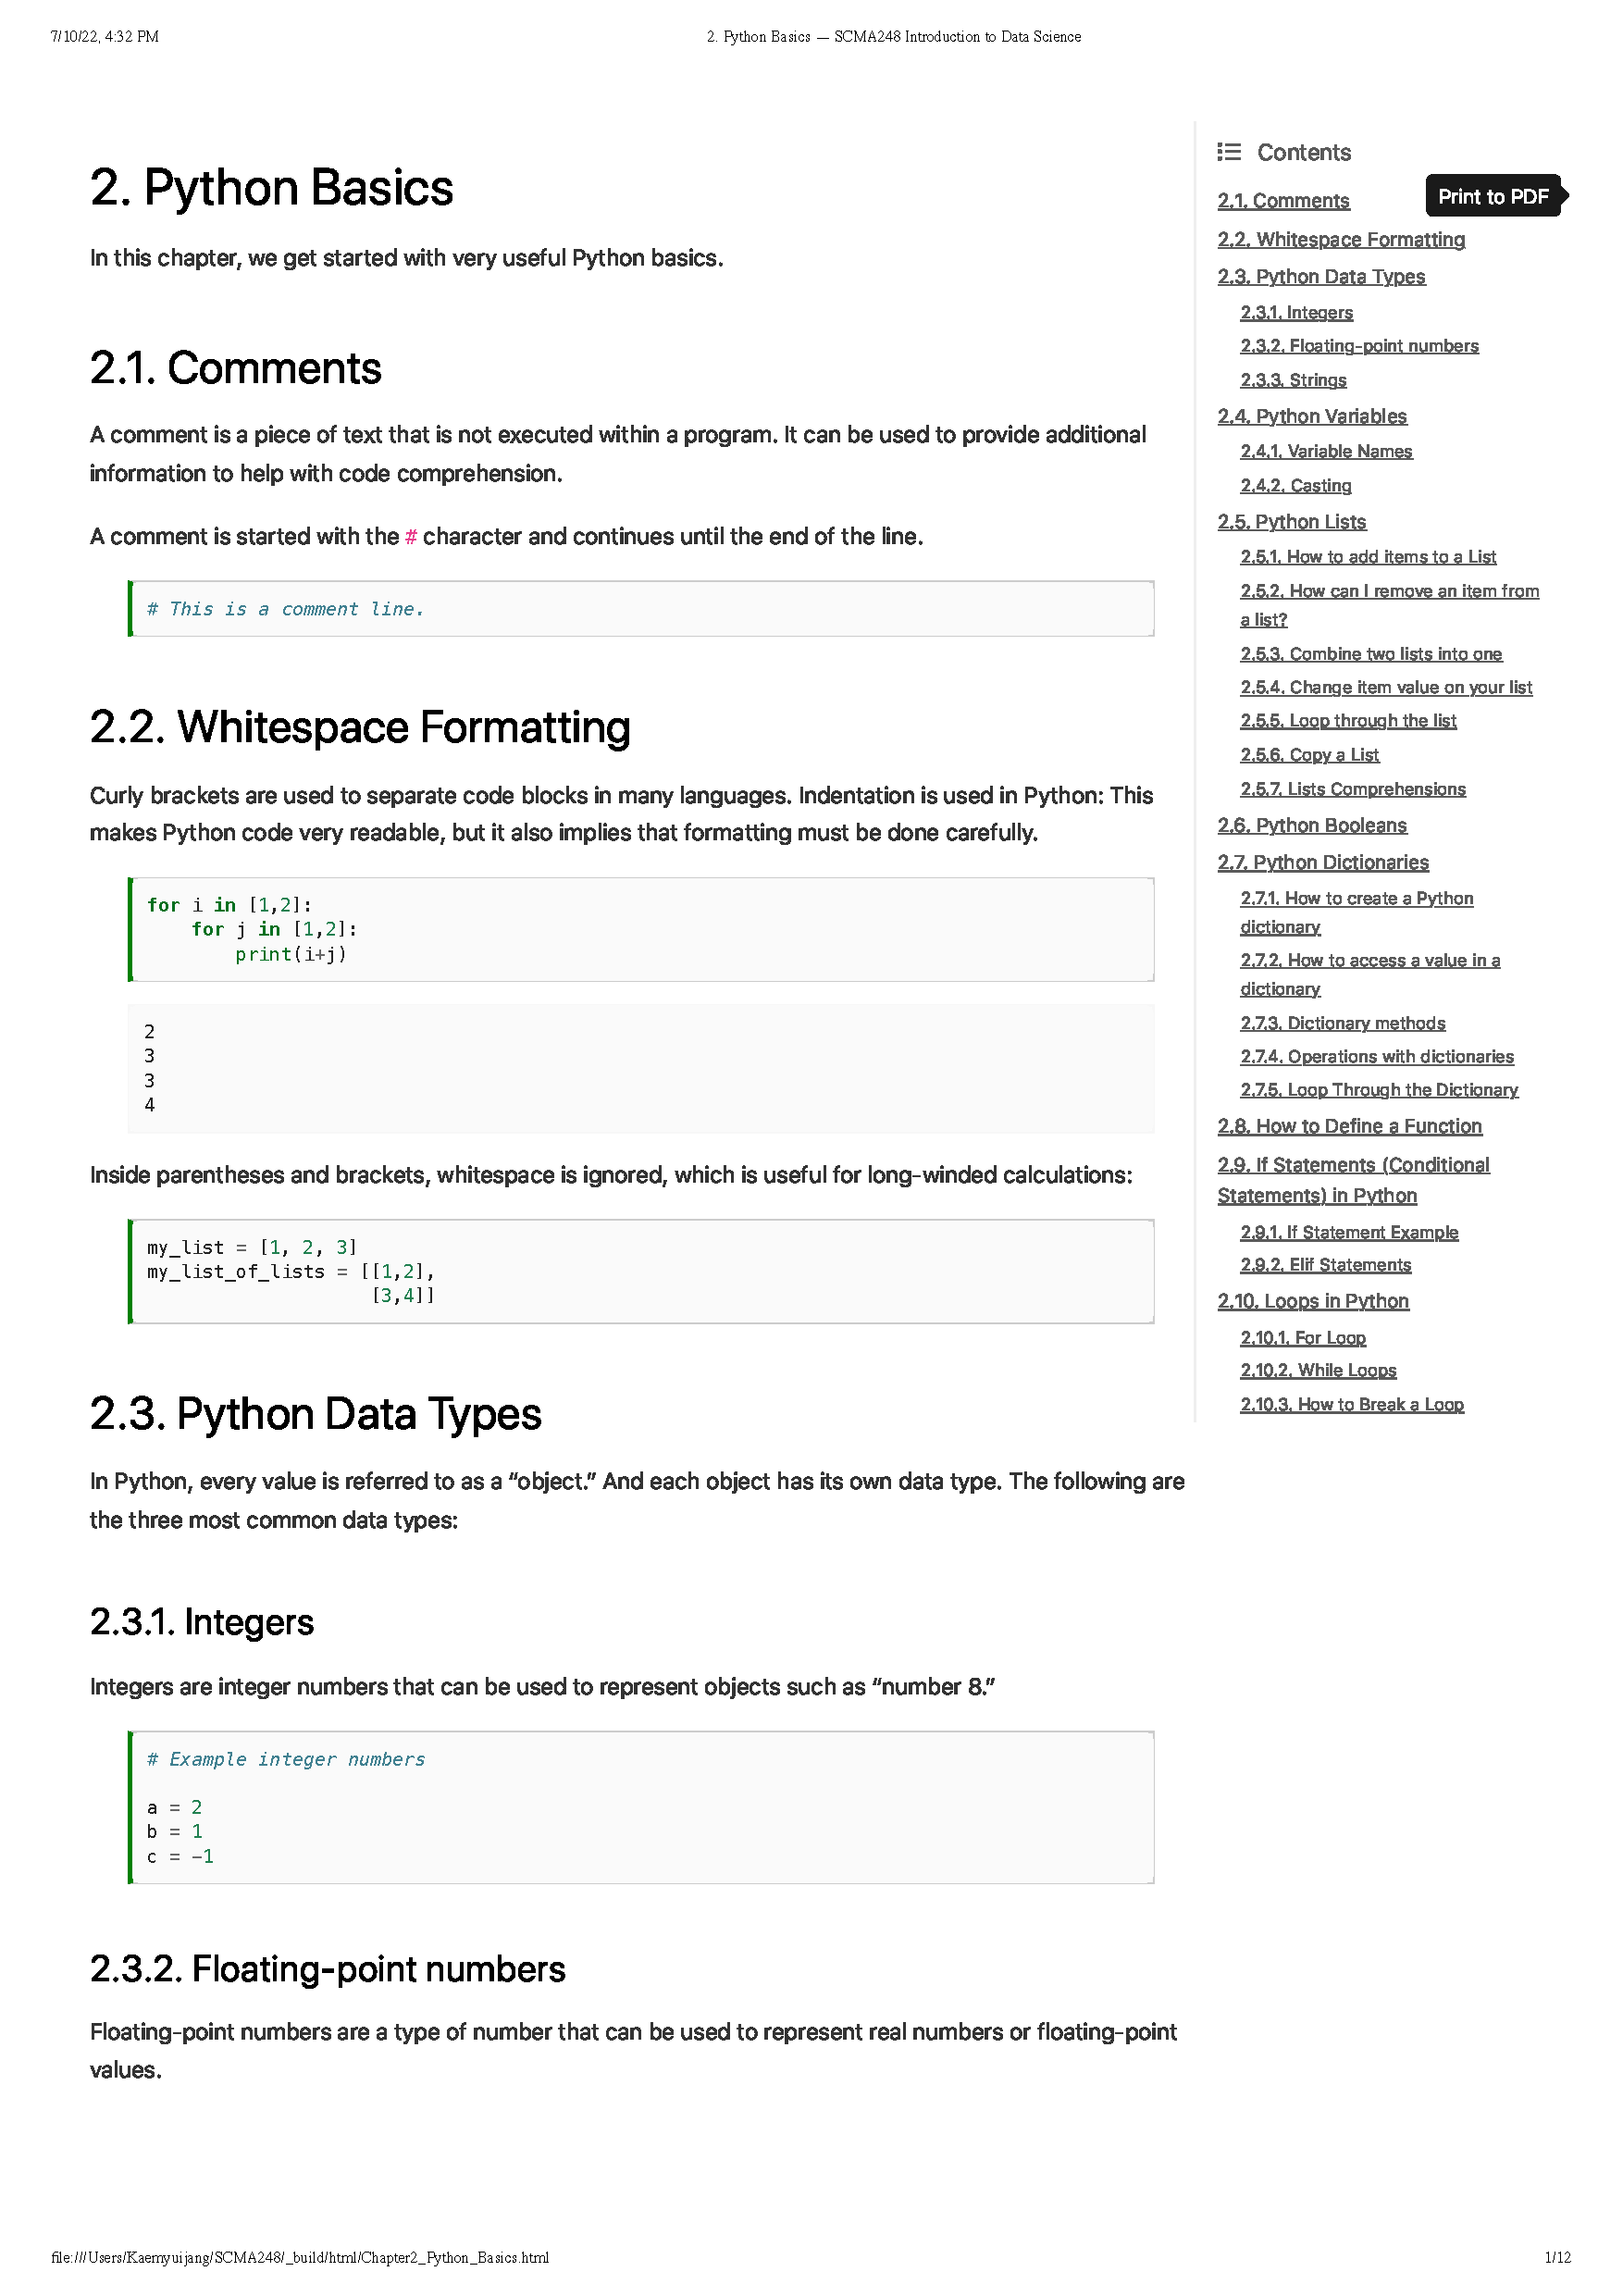
\includepdf[pages={1-},scale=1,pagecommand={\thispagestyle{plain}}, angle=0]{2Basics.pdf}
\section{Data Preparation}
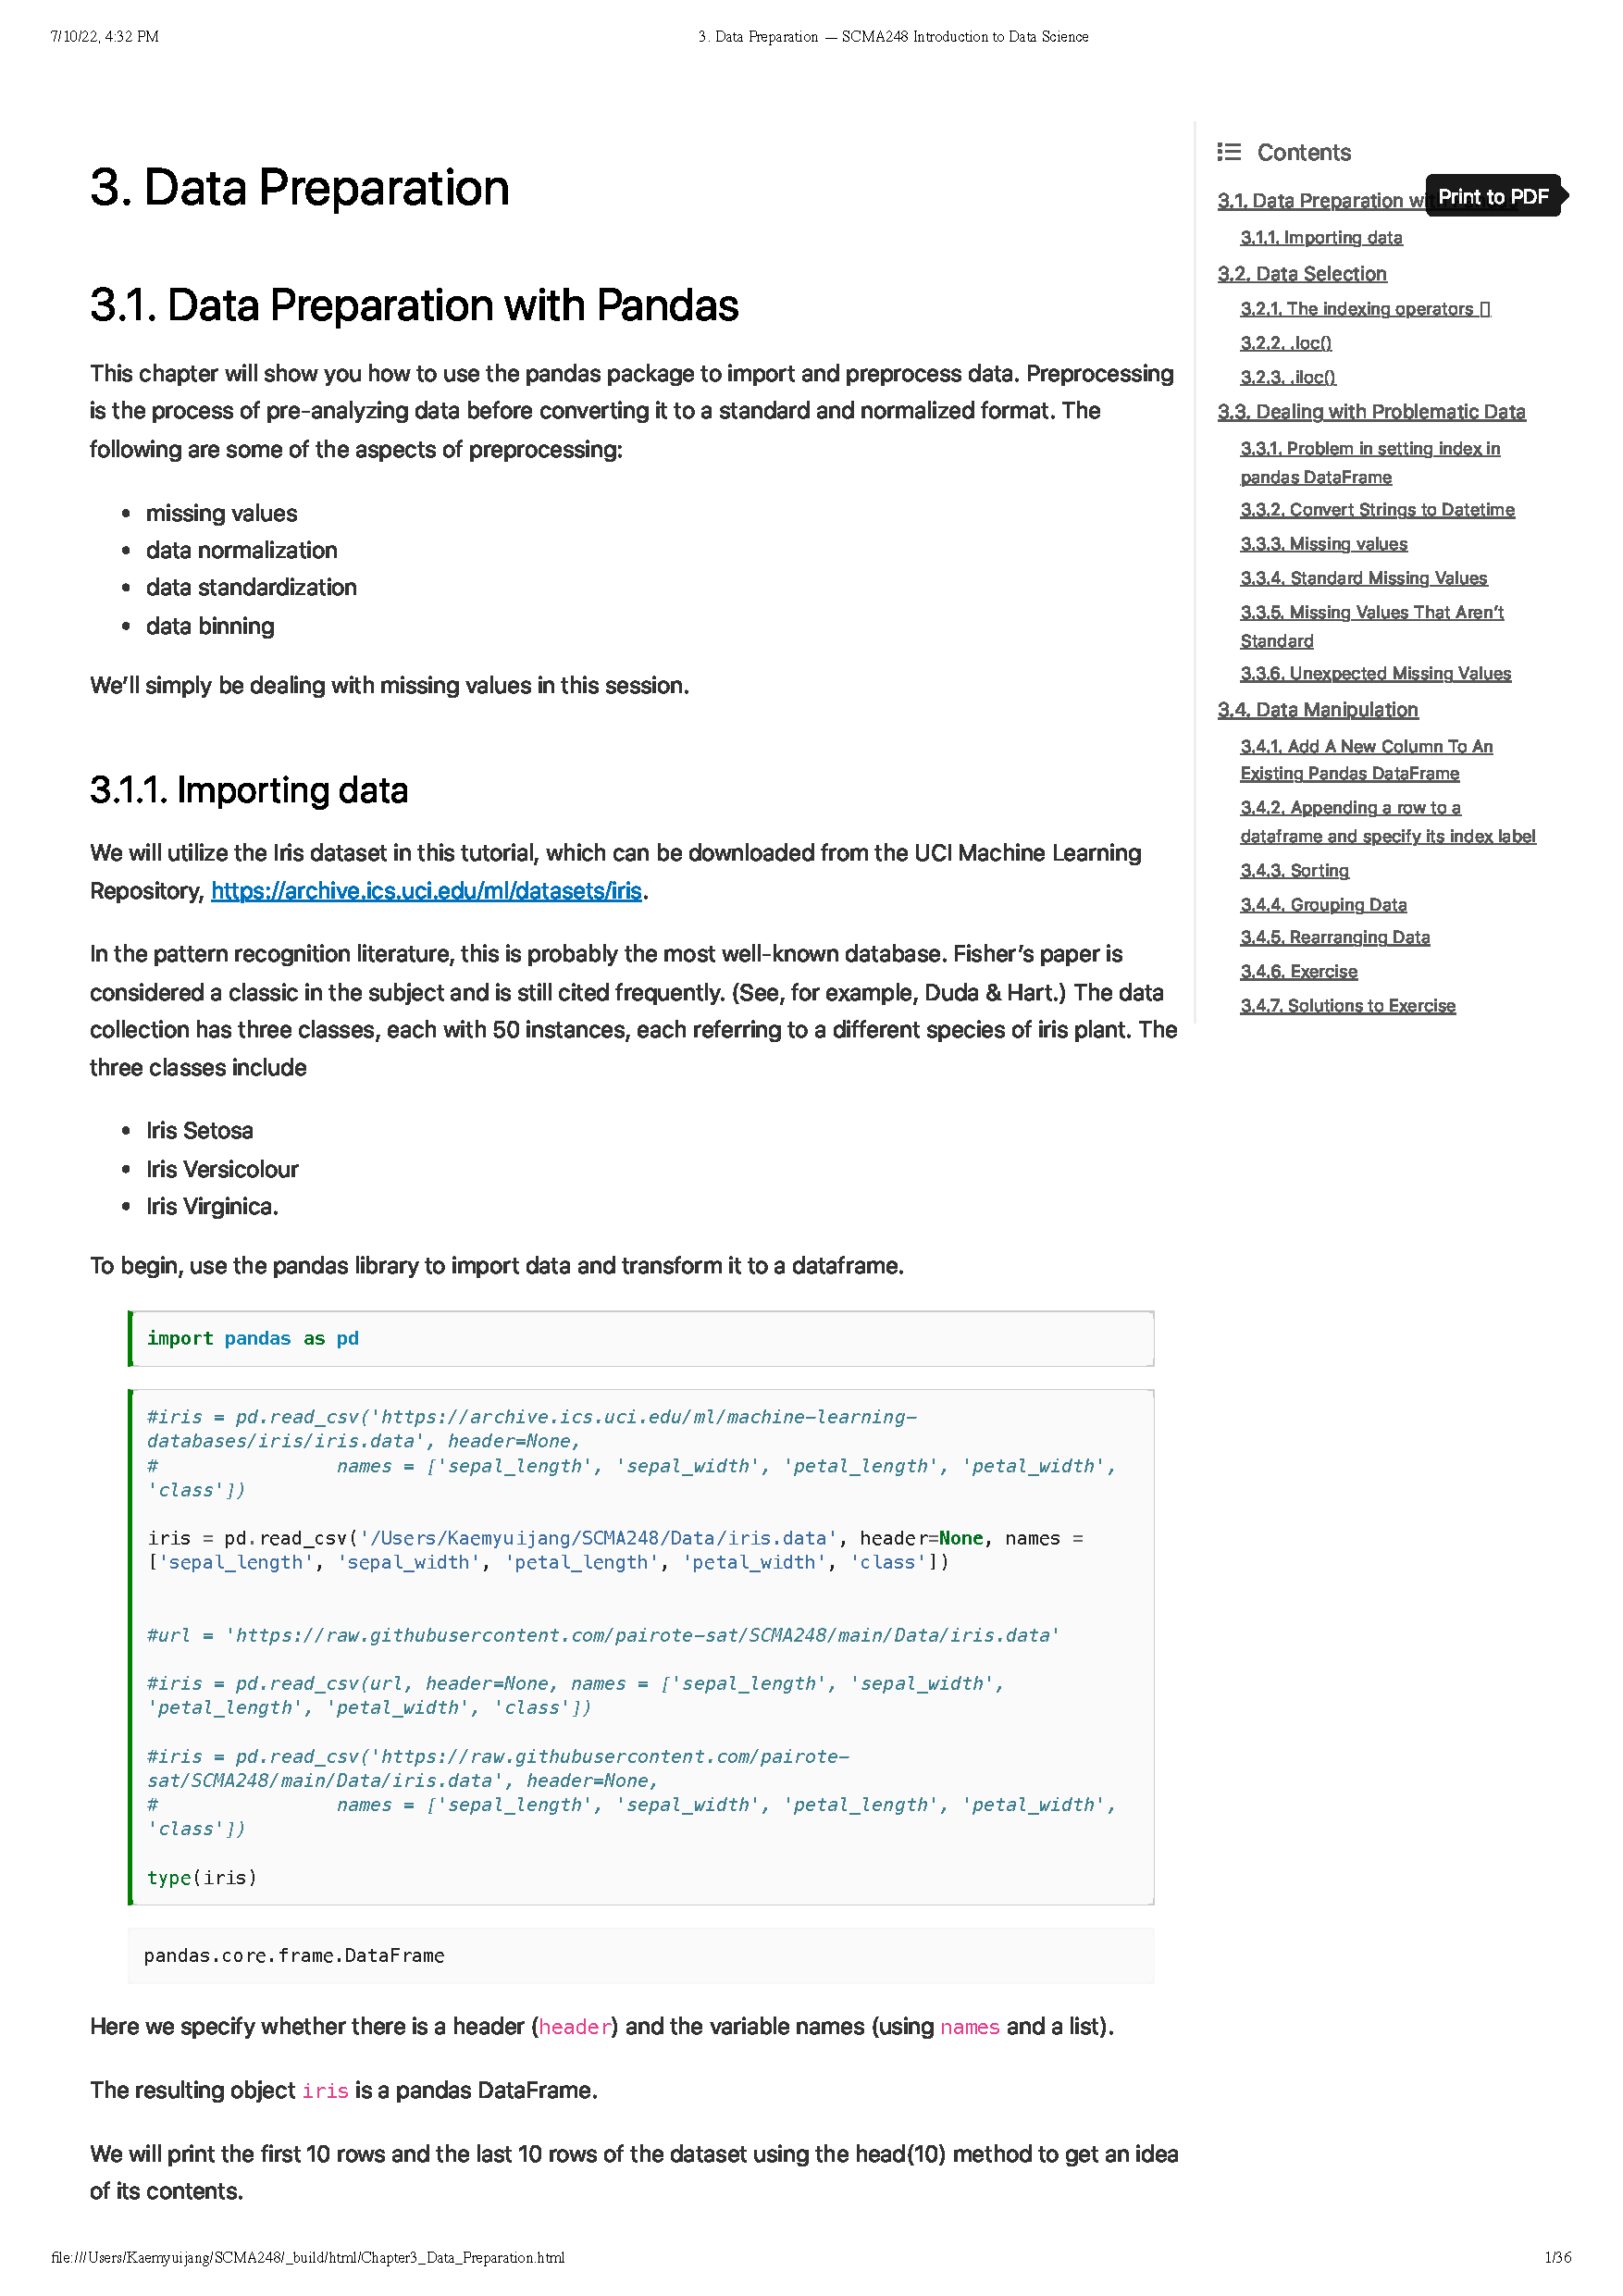
\includepdf[pages={1-},scale=1,pagecommand={\thispagestyle{plain}}, angle=0]{3Preparation.pdf}
\section{Data Visualization}
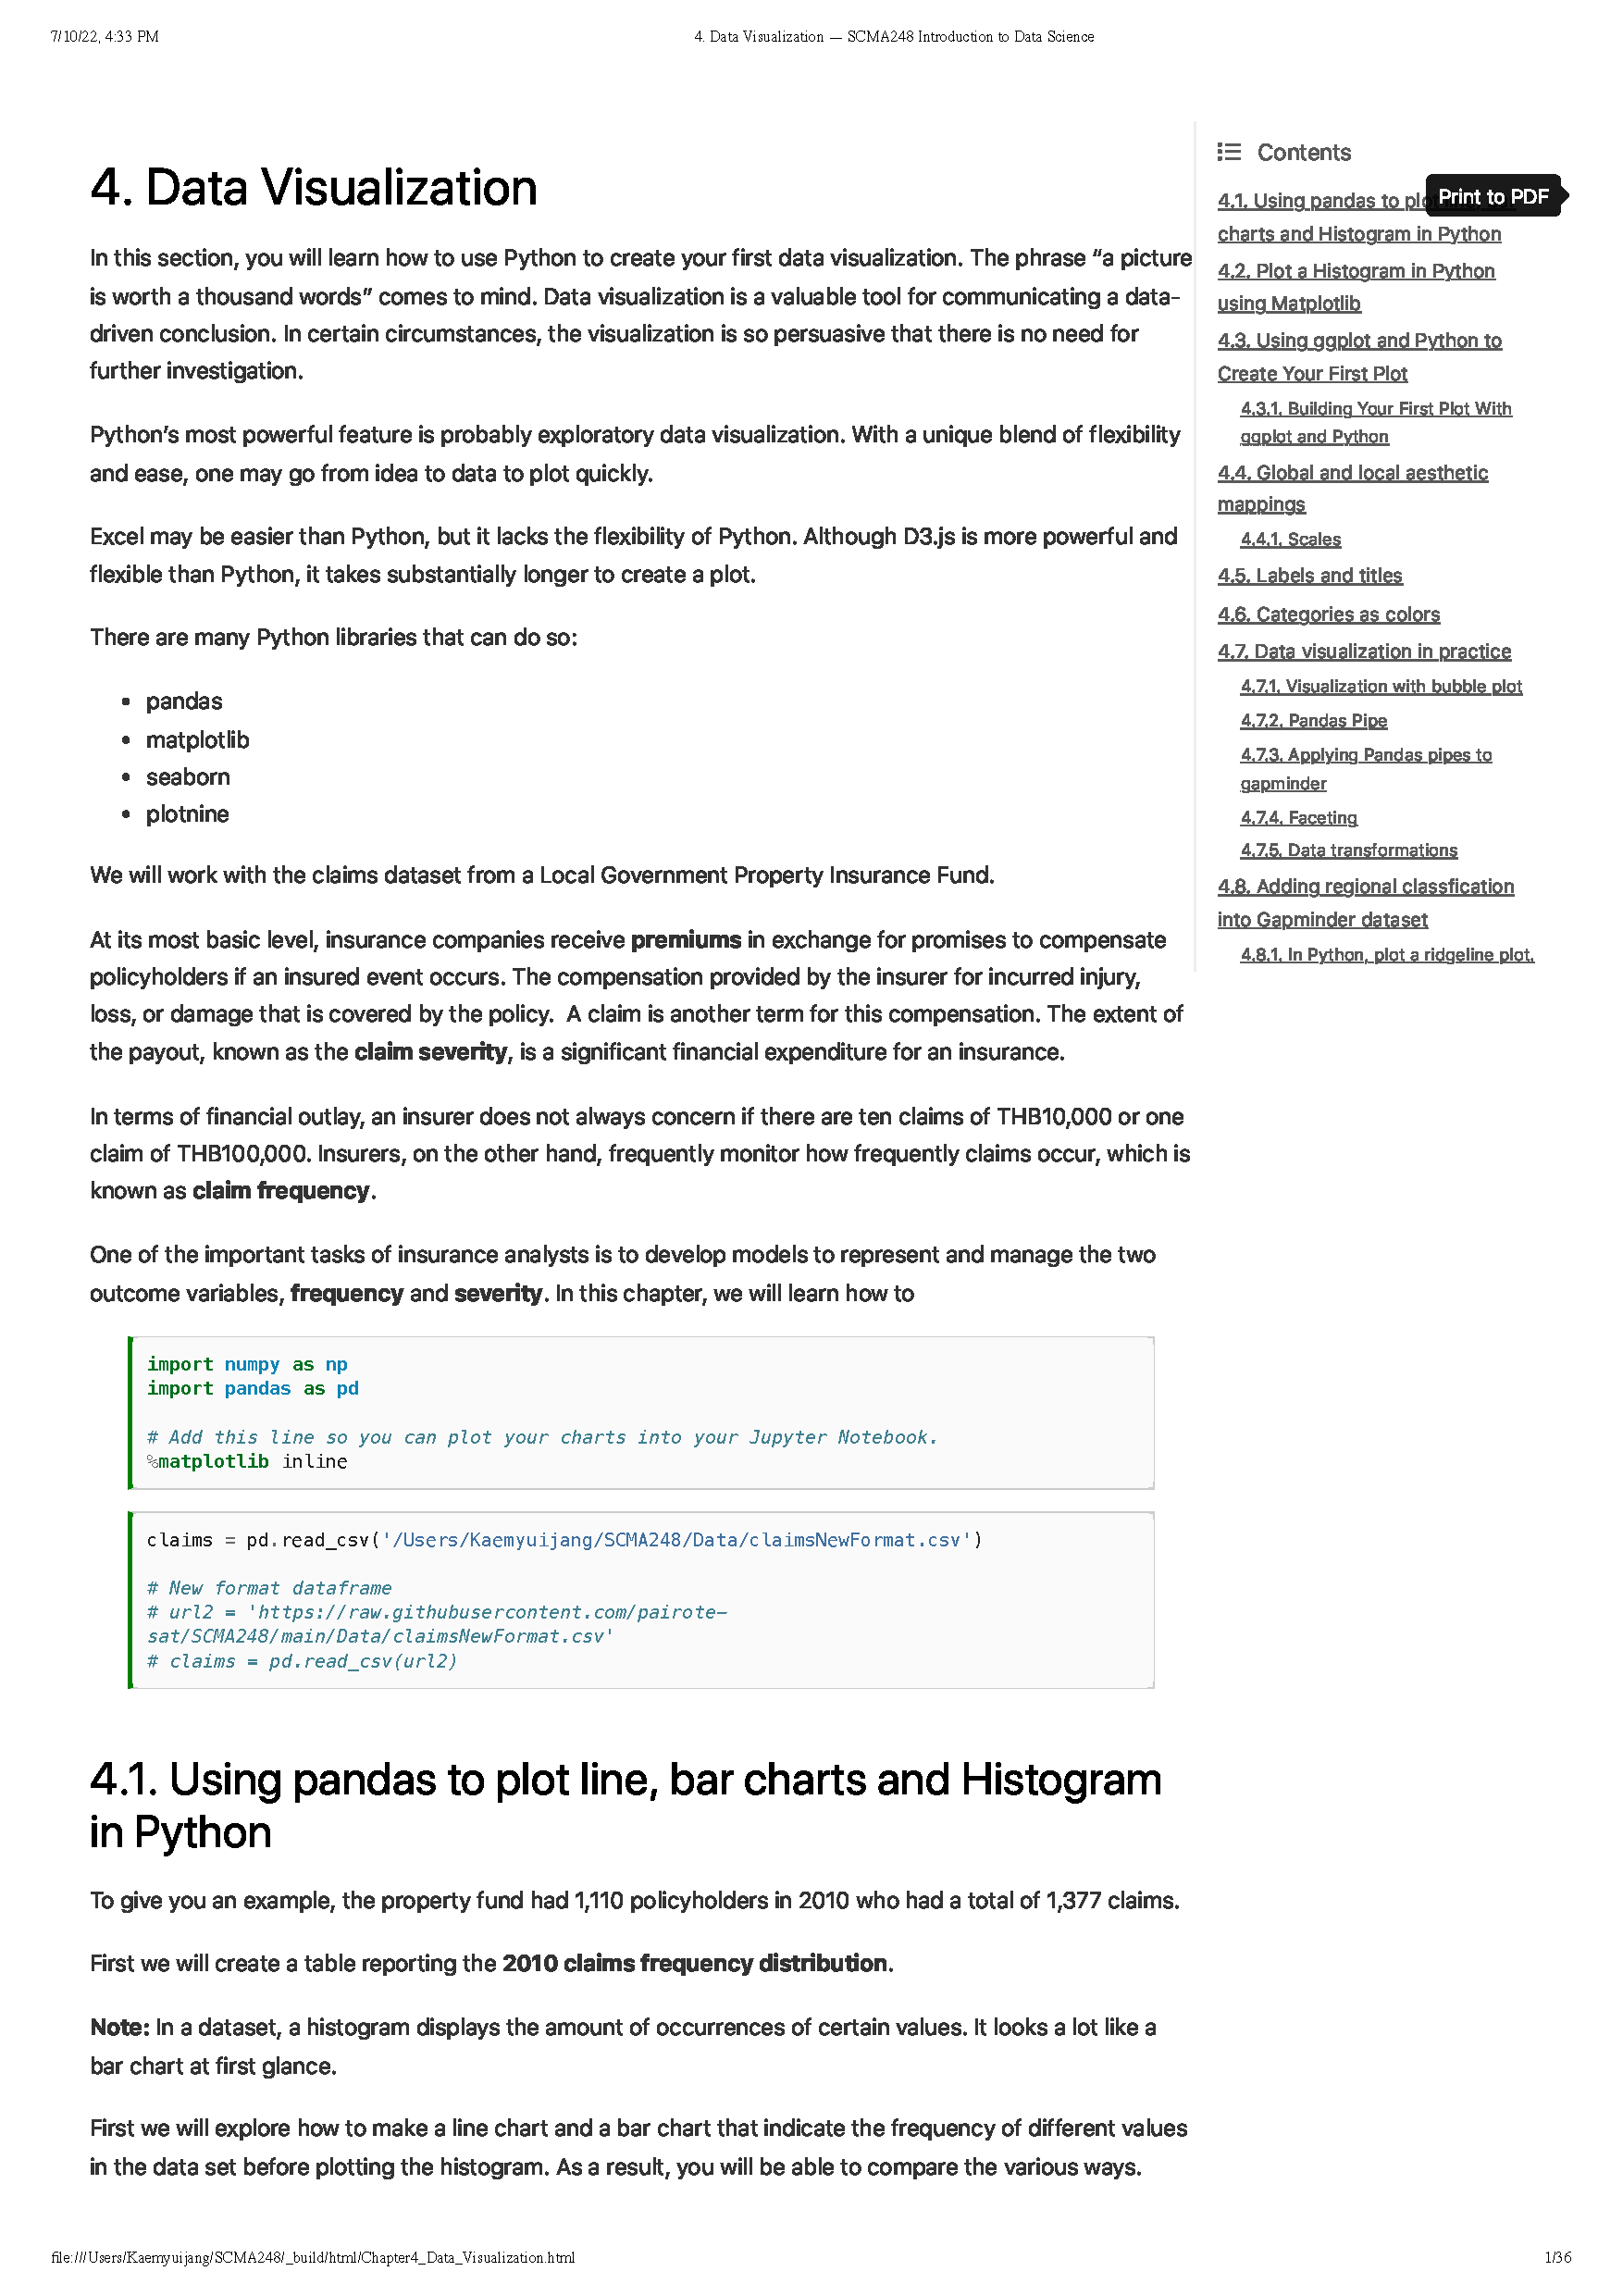
\includepdf[pages={1-},scale=1,pagecommand={\thispagestyle{plain}}, angle=0]{4Visualization.pdf}
\section{Practical Statistics}
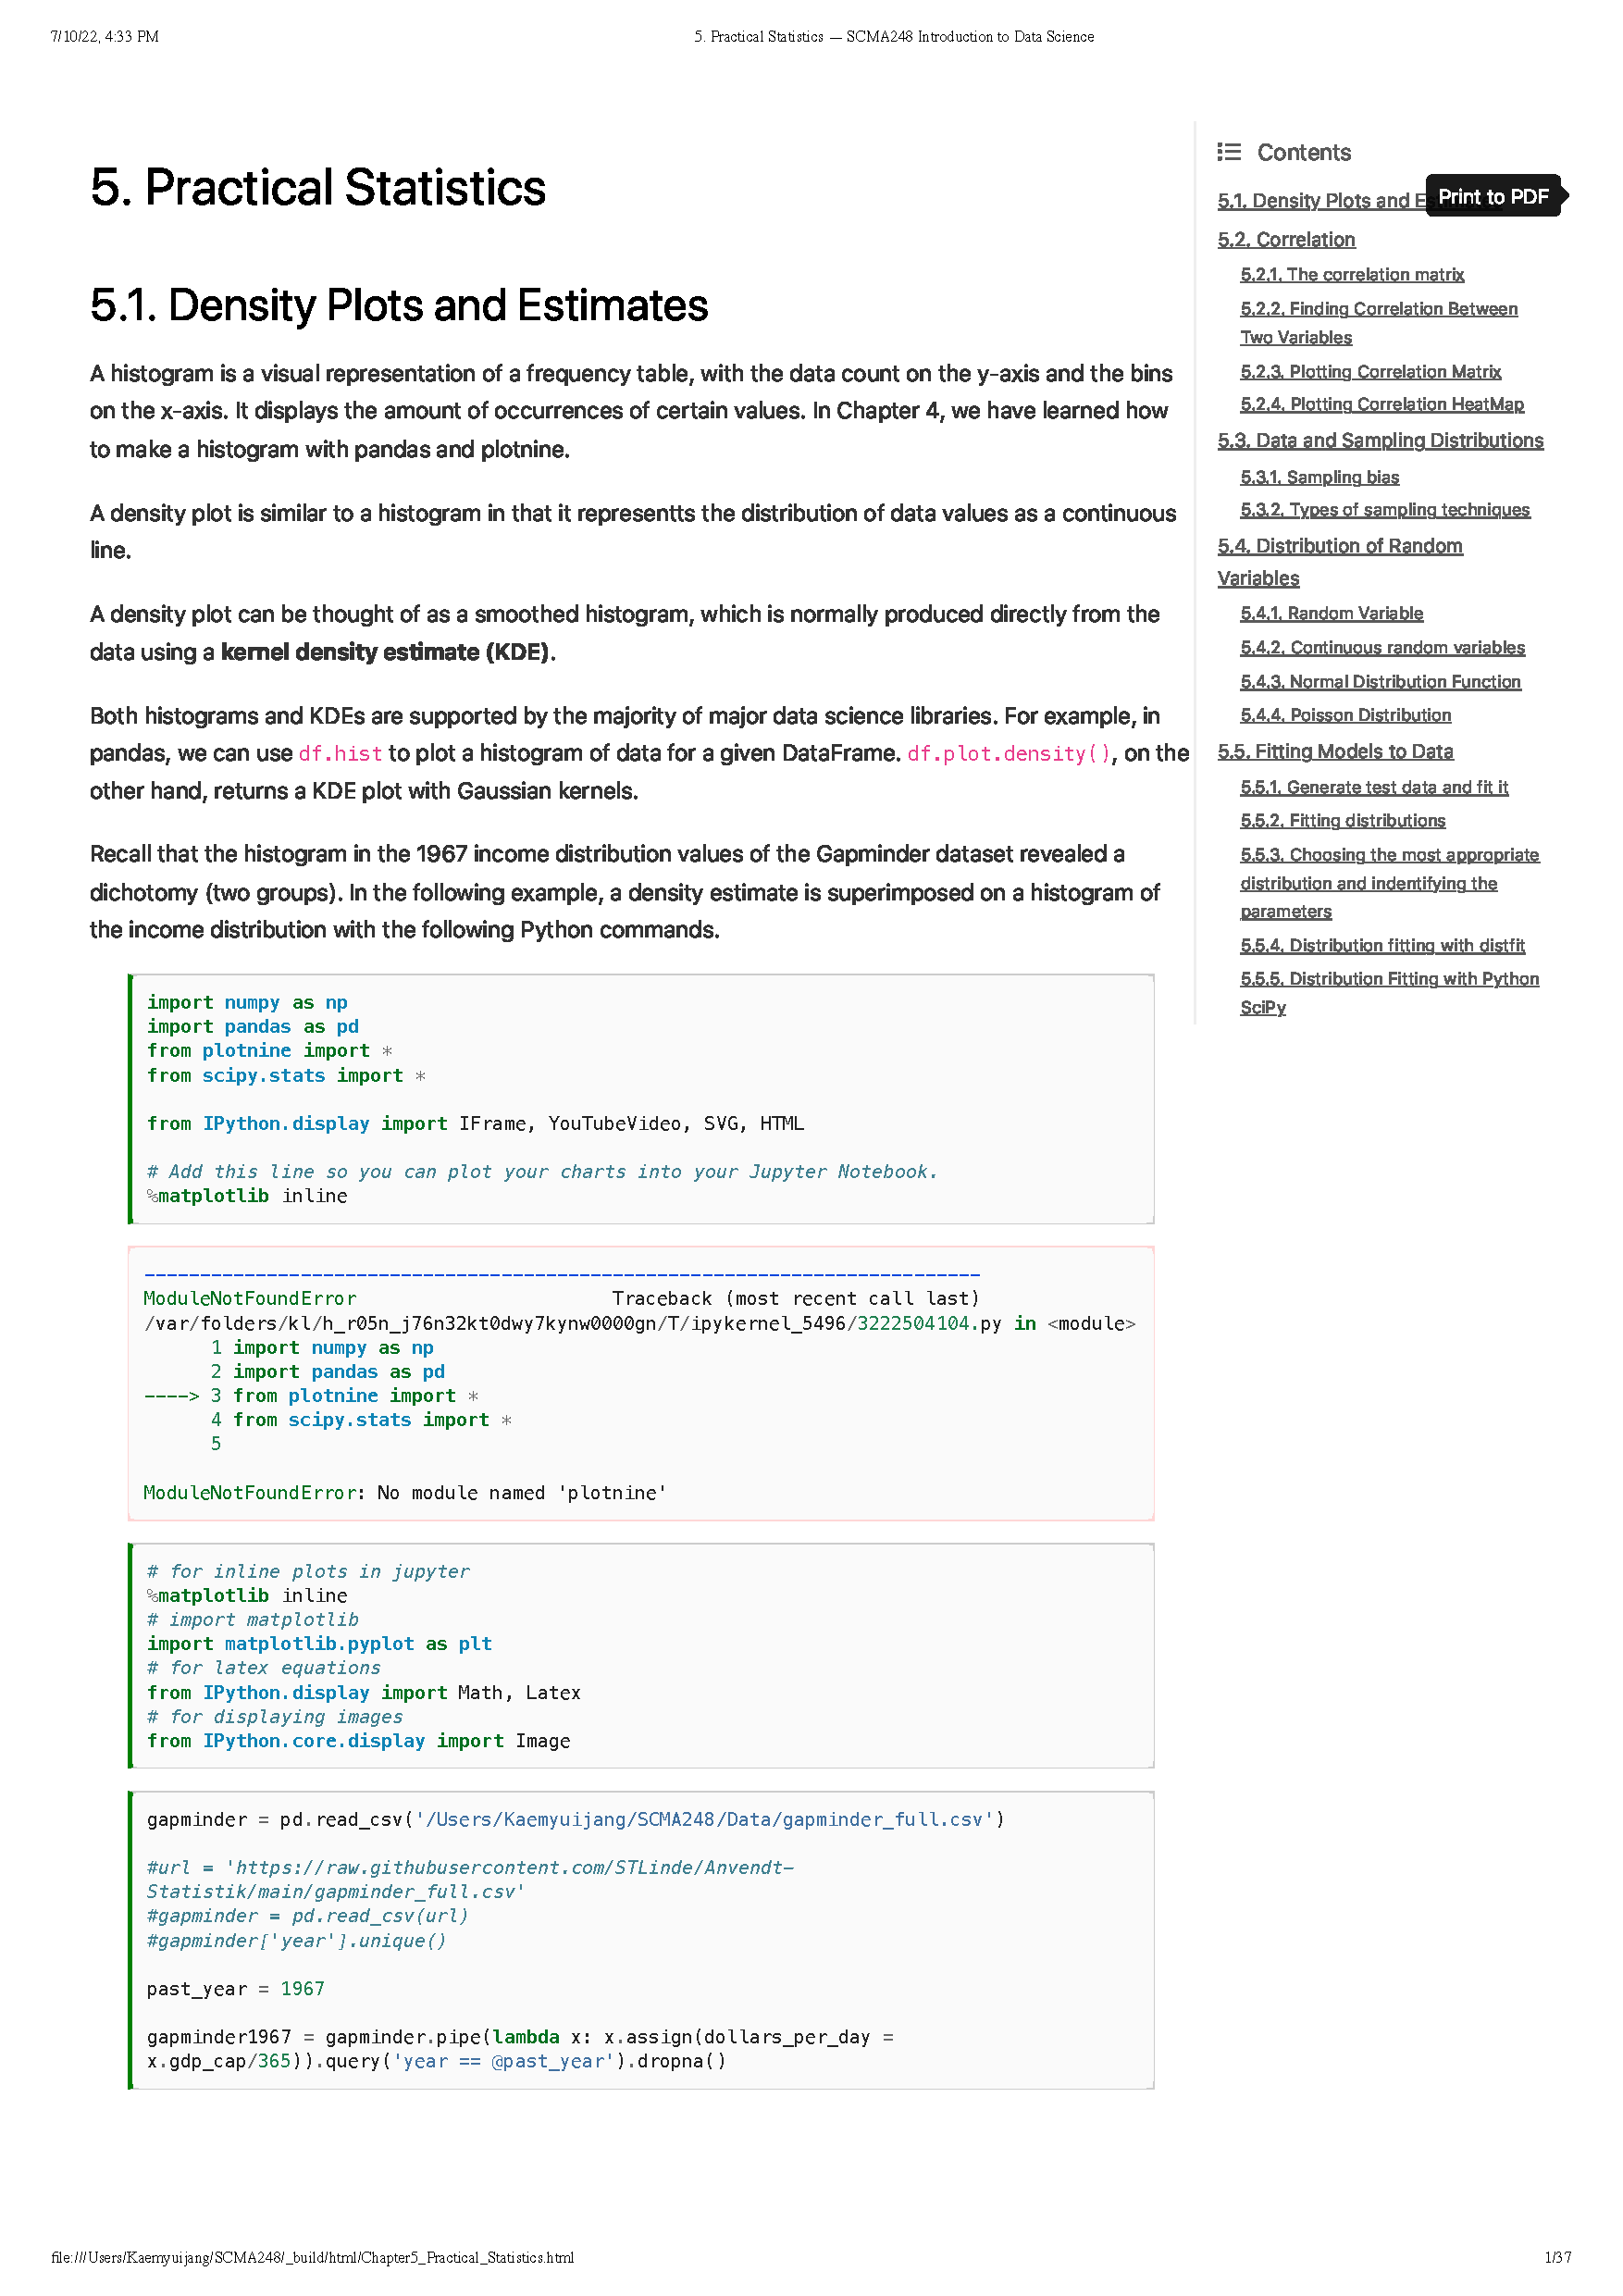
\includepdf[pages={1-},scale=1,pagecommand={\thispagestyle{plain}}, angle=0]{5Statistics.pdf}
\section{Regression Analysis}
\includepdf[pages={1-},scale=1,pagecommand={\thispagestyle{plain}}, angle=0]{6Regression.pdf}
\section{Machine learning: Introduction}
\includepdf[pages={1-},scale=1,pagecommand={\thispagestyle{plain}}, angle=0]{7Machine.pdf}
\section{Unsupervised Machine Learning: K-means Clustering}
\includepdf[pages={1-},scale=1,pagecommand={\thispagestyle{plain}}, angle=0]{8Unsupervised.pdf}

\end{document}